\documentclass[11pt,twocolumn]{article}
\usepackage{fullpage}
\usepackage[font={small,it}]{caption}
\usepackage{graphicx}
\usepackage{dcolumn}
\usepackage{bm}
\usepackage{abstract}


\begin {document}
\begin{center}

{\LARGE{\bf Broadband Imaging and Photometry on Open Star Clusters}}

{\large Tim Kornish}

University of Montana

November 24th, 2014
\end{center}

\paragraph{Abstract}

\ \

Observing celestial objects through several different filters offers many more analytic abilities than through one filter alone. Taking several dithered images of an open star cluster and mosaicking them to form a single large image in several filters. With a few mosaicked images in different filters, a Color-Magnitude Diagram (CMD) can be constructed showing characteristics of each star within the star cluster.

\paragraph{Introduction}

\ \

Images of stars and celestial objects can be taken around the world at any orientation and put into the program Astrometry.net. Astrometry.net shows the RA and Dec of the stars in images and will provide the information to reorient them with the World Coordinate System (WCS). Taking images with different filters shows how much light is emitted in certain wavebands. With Images in several filters a RGB color image can be produced showing visually what stars temperatures are. With different fluxes of stars per filter a Color-Magnitude Diagram can be created. Observing an open star cluster holds hundreds of stars with very similar distances from Earth and the same age shows that differences in flux are due to intrinsic properties of each star. Each star in the cluster was fitted with a aperture to acquire the counts given by the star. With the counts and known exposure time of each filter, the magnitude of each star in each filter can easily be calculated. These value are what is used to build the CMD.

\paragraph{Observations and Methods}

\ \

Images of the open star cluster NGC 6819 were taken 09-02-2014 using a 0.4m diameter telescope at the University of Montana. Beginning after civil twilight, flats were taken for later use in editing the raw images. Dithered images of NGC 6819 were taken in B,V, R broadband filters. Images of Landolt standards were also taken in each filter to acquire zero points of each filter. Images were reduced with dark subtracting and flat-fielding. After all images were reduced in each filter, Astrometry.net is used to locate the exact coordinates of the image on the sky $(Figure$ $ $1$)$. At the end of the observing run, darks were taken for image reduction.
\begin{center}
\begin{figure}
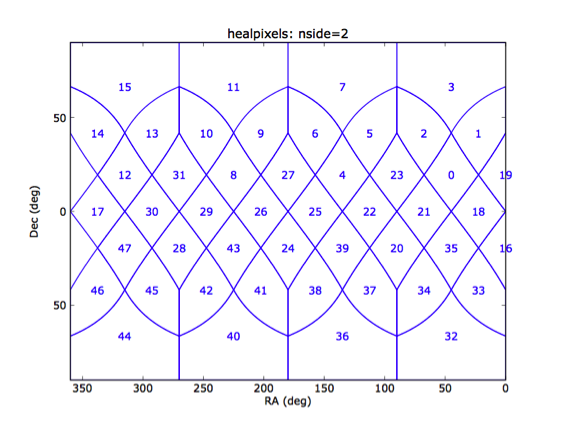
\includegraphics[scale=0.8]{Astrometry}
\caption{\small{Mapping of Astrometry.net used to locate an image in the sky taken anywhere on earth. }}
\end{figure}
\end{center}

Next was to mosaic the dithered images because the telescope used is an alt/az telescope without an installed field derotator. This causes the images to not be perfectly aligned and must be mosaicked. 

Images of NGC 6819 were taken with separate exposure times for different filters due to different saturation rates shown in $Table$ $1$.

\begin{center}
\begin{figure}
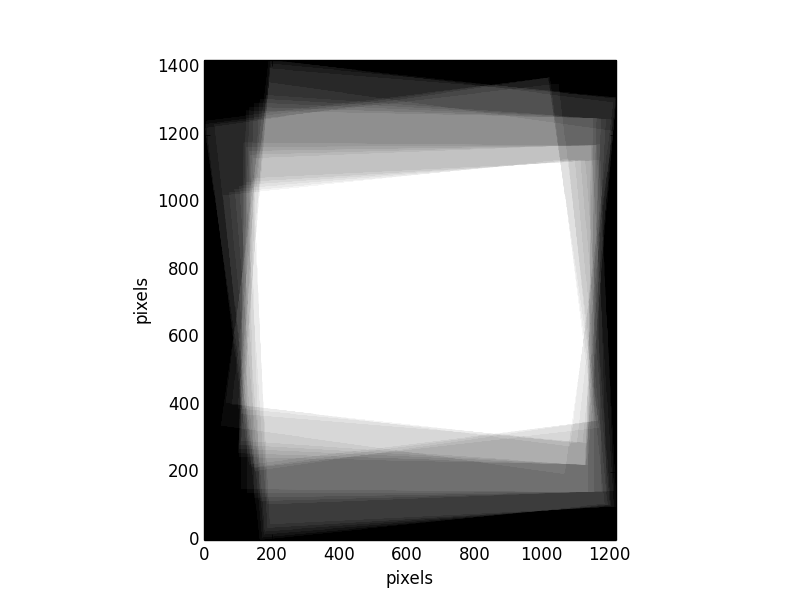
\includegraphics[scale=0.5]{figure_2}
\caption{\small{A mosaic of all the dithered images showing the motions of the telescope not perfectly tracking the open star cluster. This image shows how the actual cluster images will fit together. }}
\end{figure}
\end{center}


\begin{center}
Table 1
\end{center}
\begin{center}
\begin{tabular}{|l|l|}
\hline
\multicolumn{2}{|c|}{Filter image exposure time (s)} \\
\hline
Blue Filter & 10 \\
Red Filter & 5 \\
Visible Filter & 5 \\
\hline
\end{tabular}
\end{center}

\paragraph{Analysis}

Every image in each filter is mosaicked to build a final image with stars in the enter containing less signal-to-noise than on the outer edge. Three of these images are constructed, one per filter and then merged together to build a RGB image $(Figure$ $3)$





\begin{center}
\begin{figure}
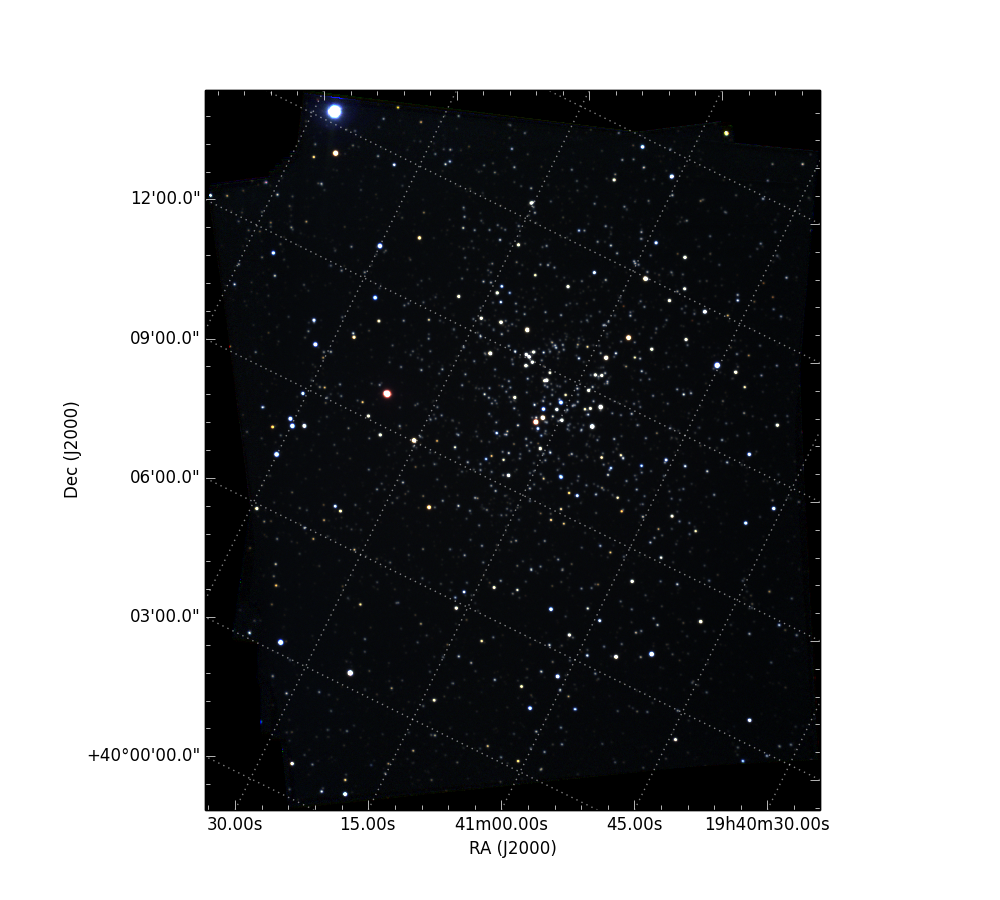
\includegraphics[scale=0.35]{figure_1}
\caption{\small{RBG color image of open star cluster NGC 6819 with RA vs. Dec coordinates labeled on the axis.}}
\end{figure}
\end{center}

With all images of the open cluster aligned in an RGB image, analysis can be done on the stars in the cluster. 
All the stars in the cluster are the same age and distance from Earth, therefore any difference in color and/or flux are intrinsic to the stars.

First the zero points of each filter must be found. This is done by analysis on three Landolt Standards. The zero points for each filter are displayed below in Table 2.

\begin{center}
Table 2
\end{center}
\begin{center} 
\begin{tabular}{|l|l|}
\hline
\multicolumn{2}{|c|}{Zero Points} \\
\hline
Blue Filter & 21.355875 $\pm$ 0.0103 \\
Red Filter & 21.775739 $\pm$ 0.0056 \\
Visible Filter & 21.670823 $\pm$ 0.0057 \\
\hline
\end{tabular}
\end{center}

\ \

With the zero points known for each filter, the magnitude of each star can be calculated in each filter. Because of the Mosaicking, some stars will be cut out and others will be excluded for not being bright enough.
$Figure$ $4$ shows a Color-Magnitude Diagram (CMD) of the stars in the open cluster. Plotting this HR diagram shows a section of the main sequence. $Figure$ $4$ only shows 511 of the stars inside the open cluster because that is all that the blue filter could find even though the visible and red filter found more as seen in $Table$ $3$. The blue filter couldn't recognize as high magnitude stars as the other filters.


\ \

\begin{center}
Table 3
\end{center}
\begin{center}
\begin{tabular}[scale=0.5]{|l|l|l|}
\hline
\multicolumn{3}{|c|}{Cluster Statistics} \\
\hline
Filter & Faintest star magnitude & Stars recognized\\ 
\hline
Blue & 16.423970 & 511\\
 
\hline
Red & 17.858989 & 1005 \\
\hline
Visible & 17.710049 & 784 \\ 
\hline
\end{tabular}

\end{center}


\begin{center}
\begin{figure}
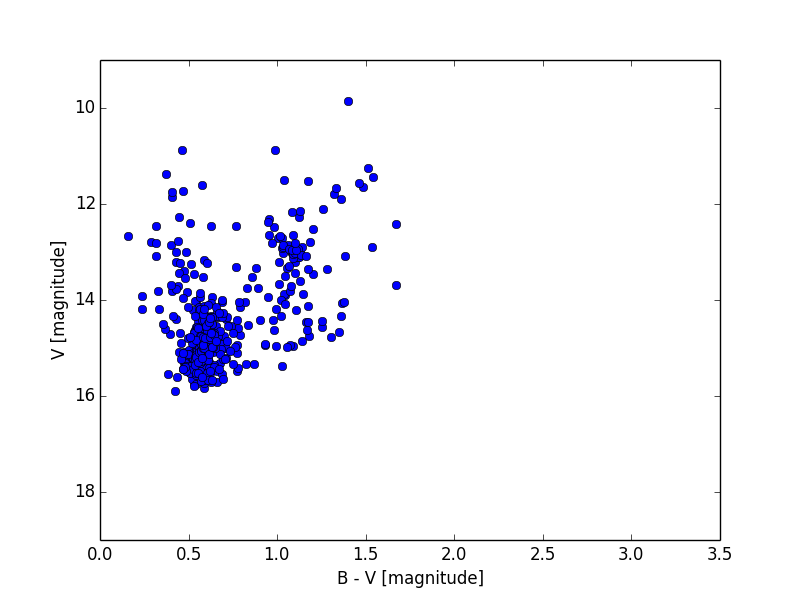
\includegraphics[scale=0.4]{figure_3}
\caption{\small{Color-Magnitude diagram of V-filter vs. (B-filter - V-filter) values on a log-log plot. These points represent stars along the main sequence. The main sequence goes up left from the bottom group. The group up to the right of the main group are giant stars diverging off from the main sequence.This shows the vast differences between hundreds of stars of the same age.}}
\end{figure}
\end{center}

The CMD shows the magnitude of stars in the V-filter vs. (B-filter - V-filter). Both axis are Log-Log scaled, B-V shows log(B) - log(V) which is also equal to: log$\frac{B}{V}$, which is directly proportional to $\frac{F_B}{F_V}$. 

\paragraph{Results}

The UM 0.4 Telescope can measure stars brightness in different filters to differing magnitudes. The Blue filter requiring longer exposure time and is less capable of seeing stars seen by the Red and Visible filter. The CMD shows the open star cluster NGC 6819 holds hundreds of stars along the main sequence with a group of giant stars that diverged from the main sequence at V-magnitude: 13.

\paragraph{Conclusion}

Open star clusters show the intrinsic properties of stars in a far easier way than observing several alone stars. Viewing through several different filters helps determine determine these properties of the stars. Using different filters requires different exposure times to saturate the same amount. With the magnitudes of the stars in the open cluster known, a CMD can be constructed showing the age and temperature of each star. The more stars and more images used, the more the CDM produces a greater defined main sequence.



\end{document}


